\section{超导序参量计算}
%\setcounter{page}{1}
%\pagestyle{plain}
接下来我们将会通过数值的方法来探索近邻效应在2D拓扑绝缘体中诱导出来的序参量的对称性,从而理解准粒子谱非对称性的起源。
\subsection{动量空间序参量计算结果}
我们在这里首先计算了拓扑绝缘体中轨道$1$在动量空间中的超导序参量$\Delta_1(\mathbf{k})$,结果如图\ref{fig19}所示,丛结果中可以看到,序参量是破坏$\mathcal{C}_4$对称性的,我们将序参量$\Delta_1(\mathbf{k})$分解成单重态通道$\Delta_s$与三重态通道$\Delta_t$,$\Delta_1(\mathbf{k})=\Delta_s(\mathbf{k})+\Delta_t(\mathbf{k})$
\begin{equation}
\begin{aligned}
\Delta_s(\mathbf{k})&=\frac{1}{2}\left[\Delta_1(\mathbf{k})+\Delta_1(\mathbf{-k})\right]\\
\Delta_t(\mathbf{k})&=\frac{1}{2}\left[\Delta_1(\mathbf{k})-\Delta_1(\mathbf{-k})\right]
\end{aligned}
\end{equation}
\begin{figure}[h]
\centering
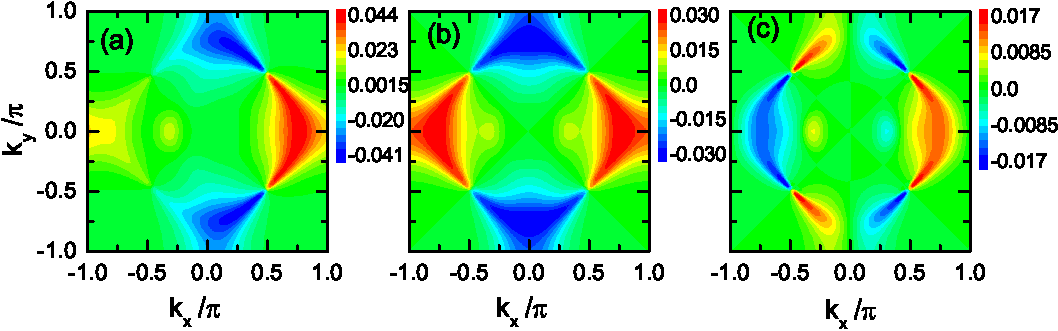
\includegraphics[scale=0.7]{pic/fig20}
\caption{(a)轨道1的超导序参量(b)轨道1单重态通道的序参量(c)轨道1三重态通道的序参量}\label{fig19}
\end{figure}
两种不同通道的序参量计算结果如图\ref{fig19}(b,c)所示,对于单重态通道$\Delta_s$,其结果与纯的$d_{x^2-y^2}$的对称性是完全相同的,但是对于三重态通道$\Delta_t$它的结果表现出了$p$-波配对的特征。所以对于2D拓扑绝缘体层轨道1,其受到超导近邻效应之后,诱导出的电子配对对称性是$d+p$-波,所以轨道1整体的的超导序参量$\Delta_1(\mathbf{k})$的$\mathcal{C}_4$对称性是破坏的,所以准粒子的谱函数的$\mathcal{C}_4$对称性同样是不存在的。同时此时超导序参量的反演对称性也是破坏的$\Delta_1(\mathbf{k})\neq\Delta_1(\mathbf{-k})$,因此在动量空间中对自旋依赖的谱函数$A_{\tau\sigma}(\mathbf{k},E)$,反演对称性也是被破坏的$A_{\tau\sigma}(\mathbf{k},E)\neq A_{\tau\sigma}(-\mathbf{k},E)$。另一方面,由于体系存在时间反演对称性,所以谱函数满足$A_{\tau\uparrow}(\mathbf{k},E)\equiv A_{\tau\downarrow}(-\mathbf{k},E)$,因此对于整个的谱函数,反演对称性是存在的,计算结果如图\ref{fig16}所示。
%============================================
\subsection{实空间序参量计算结果}
接下来,我们计算了在实空间中,同时沿$x$与$y$方向同时考虑开边界条件情况下,与格点位置依赖的轨道1对应的$d$-波超导序参量$\Delta_1(i)$,结果如图\ref{fig20}(a)所示,我们同时计算了四个边界上的序参量,结果如图\ref{fig20}(b)所示。
\begin{figure}[h]
	\centering
	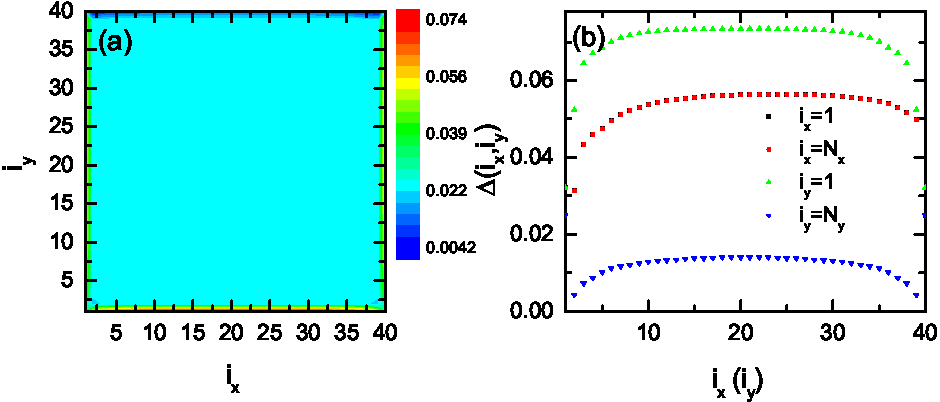
\includegraphics[scale=0.9]{pic/fig21}
	\caption{(a)2D拓扑绝缘体轨道1实空间中的$d$-波序参量(b)实空间四条边界上的$d$-波序参量分布}\label{fig20}
\end{figure}

从上面的结果中可以看到,在$i_y=1$这个边界上,序参量的值相对比较大,但是在$i_y=N_y$边界上,序参量幅值是非常小的,因此在这条边上,在圆柱形结构中,存在拓扑保护的无能隙的边界态,这与我们前面计算谱函数得到的结论是完全一致的。同时,对于一个开边界有限大小的体系,上边界几乎为零的$d$-波序参量也是其无法在拐角处形成束缚态的的原因。因为按照第一章的有效边界理论分析,正是因为$d$-波配对在不同方向上的符号相反,可以在相邻的边界上形成质量畴壁,从而在质量反号的交界处形成零能束缚态,而上边界上诱导出有效的$d$-波序参量是非常小的,所以无法在该边界与相邻边界形成质量畴壁,因而只能在下边界与相邻边界的拐角处形成马约拉纳拐角态,即图\ref{fig18}(c)计算结果所示。这里需要强调的是,上边界通过近邻效应诱导的超导能隙非常小这个结论是非常普适的,即使在一定范围内改变体系的化学势,结果仍然保持不变。
%============================================
\subsection{本章总结}
本章中,我们主要计算了实空间与动量空间中,在2D拓扑绝缘体中诱导出的超导配对的对称性问题。从动量空间中的计算可以看到,层间耦合导致在2D拓扑绝缘体中诱导的电子配对不仅仅具有和底层$d$-波超导体相同对称性的分量,同时也会诱导出$p$-波分量,这两种不同对称形式的配对在动量空间中混合之后就会破坏原有的$\mathcal{C}_4$对称性,因此相比较于将电子配对唯象的处理为拓扑绝缘体的本征属性,此时会对马约拉纳拐角态出现的位置有一些较大的影响。在实空间中$d$-波序参量的计算结果也表明,在不同的边界上诱导出来的能隙也是不相同的。上边界诱导的$d$-波配对幅值较小,所以无法打开边界态能隙,从而无法在上边界于其相邻边界的拐角处形成马约拉纳拐角态。这些序参量分析的结果于前面谱函数及能带计算的结果都是相互符合的。







